\chapter{Schnittstellen}

Ein wichtiger Bestandteil des TourLive Gesamtsystems ist die Kommunikation zwischen den verschiedenen Komponenten. 

Die Schnittstellen werden in private und öffentlichen Schnittstellen unterteilt. Über die privaten Schnittstellen kommunizieren die TourLive Geräte (Aufnahmegeräte und der RadioTourSpeaker) mit dem TourLive Server und dem Device Management Server. Die öffentlichen Schnittstellen dienen Drittentwicklern zur Abfrage von TourLive Daten. 

\section{Private Schnittstellen}
Folgende Abbildung bietet eine grobe Übersicht über alle verfügbaren privaten Schnittstellen.
\begin{figure}[H]
	\centering
	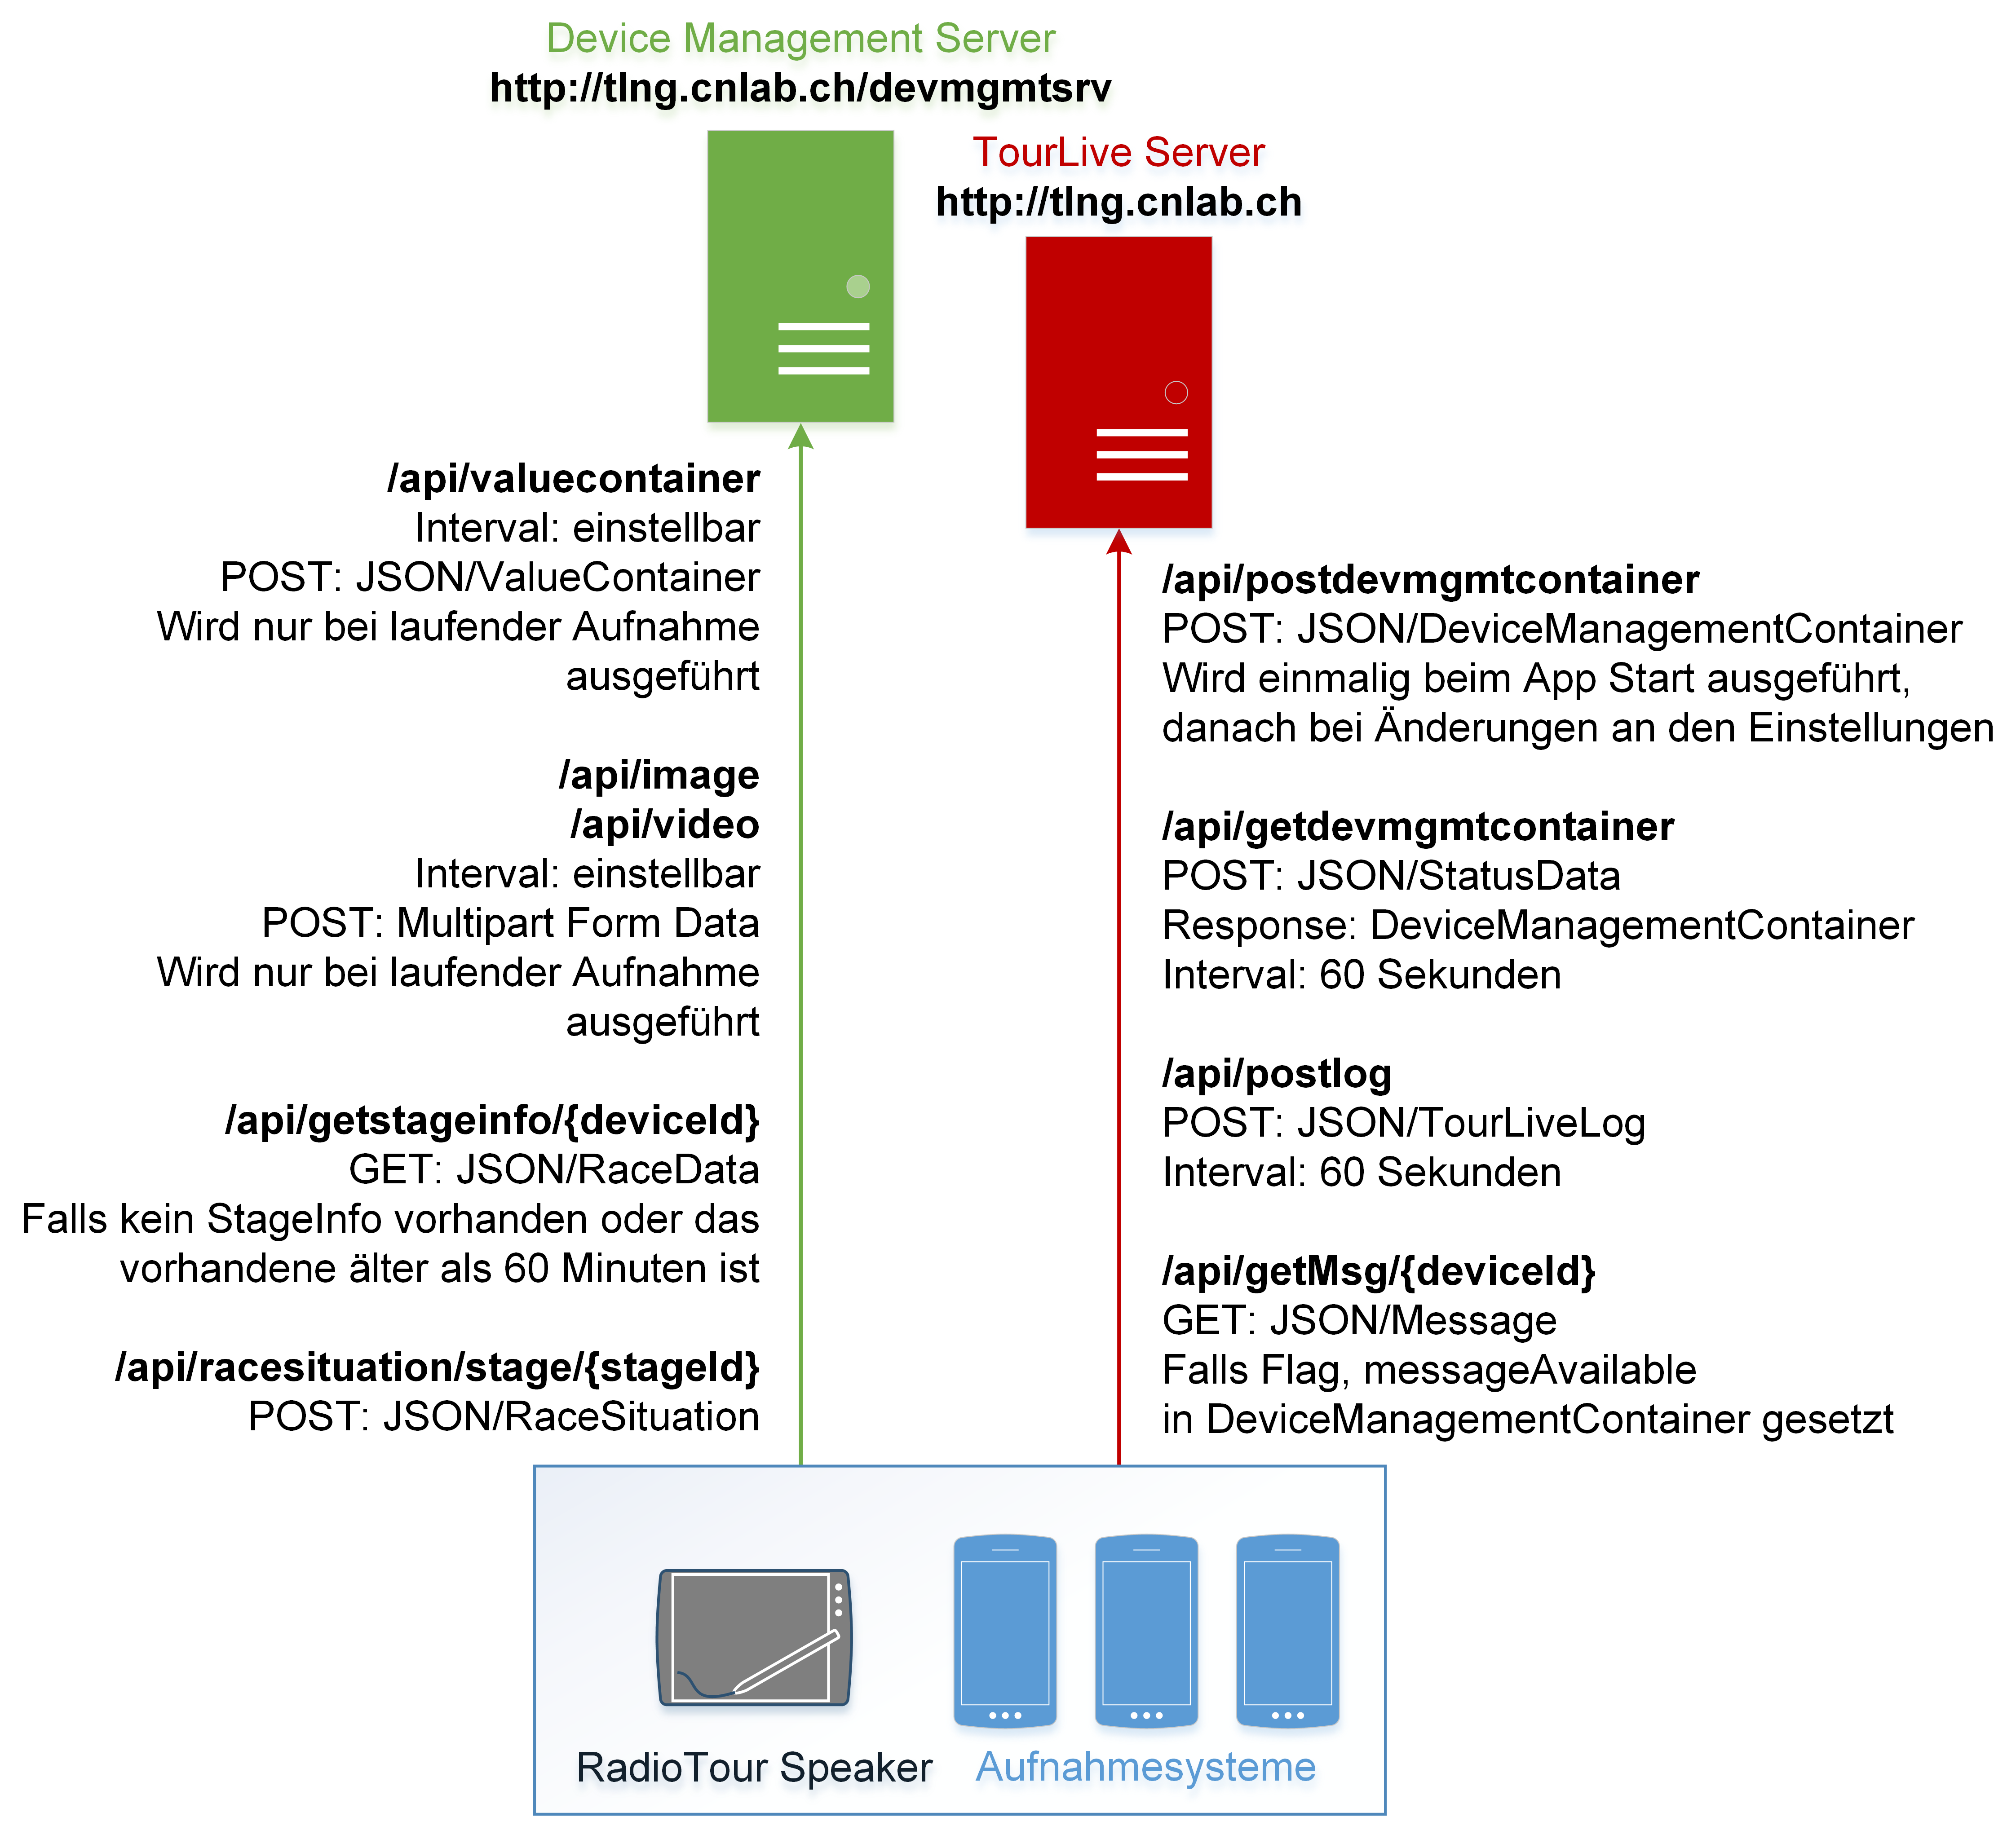
\includegraphics[width=130mm]{images/uebersicht_schnittstelle.png}
	\caption{Übersicht private Schnittstellen}
\end{figure}

\subsection{Schnittstellen TourLive Server}
\label{sec:tourliveserverapi}

Die Aufnahmegeräte liefern über diese Schnittstellen ValueContainer, Bilder und Videos an den TourLive Server.

\subsubsection{ValueContainer an den TourLive Server senden}
\begin{longtable}{ p{2.5cm} p{3.5cm} p{6cm}}
	\textbf{URL:} & \multicolumn{2}{p{10cm}}{/api/valuecontainer} \\
	\textbf{Request:} & Method: & POST \\
		& Content-Type: & application/json \\
		& Body: & JSON-String \textit{ValueContainer}\\
	\textbf{Response:} & Header: & HTTP/1.1 200 OK \\
		& Body: & <empty> \\
	\textbf{Zeitpunkt:} & \multicolumn{2}{p{10cm}}{Bei laufender Aufnahme} \\ 
	\textbf{Interval:} & \multicolumn{2}{p{10cm}}{konfigurierbar} \\ 
	\caption{Schnittstelle ValueContainer}
\end{longtable}

\paragraph{JSON Beispiel - ValueContainer}
Der TourLive Server erwartet das folgende JSON-Struktur für die Darstellung eines ValueContainers.

\begin{figure}[htb]
	\centering
	\lstinputlisting[language=json]{jsonfiles/valueContainer.json}
	\caption{JSON-Struktur: ValueContainer}
	\label{fig:valuecontainer}
\end{figure}

\subsubsection{Bild an den TourLive Server senden}
\begin{longtable}{ p{2.5cm} p{3.5cm} p{6cm}}
	\textbf{URL:} & \multicolumn{2}{p{10cm}}{/api/image} \\
	\textbf{Request:} & Method: & POST \\
		& Content-Type: & multipart/form-data [3 Boundaries] \\
		& Body-Boundary 1: & text/plain (timestamp) \\
		& Body-Boundary 2: & text/plain (deviceId) \\
		& Body-Boundary 3: & application/octet-stream (Bild) \\
	\textbf{Response:} & Header: & HTTP/1.1 200 OK \\
		& Body: & <empty> \\
	\textbf{Zeitpunkt:} & \multicolumn{2}{p{10cm}}{Bei laufender Aufnahme, falls Image aktiviert ist} \\ 
	\textbf{Interval:} & \multicolumn{2}{p{10cm}}{konfigurierbar}
\end{longtable}

\subsubsection{Video an den TourLive Server senden}
\begin{longtable}{ p{2.5cm} p{3.5cm} p{6cm}}
	\textbf{URL:} & \multicolumn{2}{p{10cm}}{/api/video} \\
	\textbf{Request:} & Method: & POST \\
		& Content-Type: & multipart/form-data [3 Boundaries] \\
		& Body-Boundary 1: & text/plain (timestamp) \\
		& Body-Boundary 2: & text/plain (deviceId) \\
		& Body-Boundary 3: & application/octet-stream (Video) \\
	\textbf{Response:} & Header: & HTTP/1.1 200 OK \\
		& Body: & <empty> \\
	\textbf{Zeitpunkt:} & \multicolumn{2}{p{10cm}}{Bei laufender Aufnahme, falls der Videostream aktiviert ist} \\ 
	\textbf{Interval:} & \multicolumn{2}{p{10cm}}{konfigurierbar} 
\end{longtable}

\subsubsection{Rennsituation an dn TourLive Server senden}
\begin{longtable}{ p{2.5cm} p{3.5cm} p{6cm}}
	\textbf{URL:} & \multicolumn{2}{p{10cm}}{/api/racesituation/stage/\{stageId\}} \\
	\textbf{Request:} & Method: & POST \\
		& Body: & JSON-String 'RaceSituation'\\	
	\textbf{Response:} & Header: & HTTP/1.1 200 OK \\
		& Body: & <empty> \\	
	\textbf{Bemerkung:} & \multicolumn{2}{p{10cm}}{Der RadioTourSpeaker sendet (unabhängig von den TourLive Aufnahmegeräten) periodisch die Rennsituation an den Server}
\end{longtable}

\paragraph{JSON Beispiel - RaceSituation}
Der TourLive Server erwartet das folgende JSON-Struktur für die Darstellung der Rennsituation.
\begin{figure}[H]
	\centering
	\lstinputlisting[language=json]{jsonfiles/raceSituation.json}
	\caption{JSON-Struktur: RaceSituation}
\end{figure}

\subsection{Renninformationn vom TourLive Server abfragen}
\begin{longtable}{ p{2.5cm} p{3.5cm} p{6cm}}
	\textbf{URL:} & \multicolumn{2}{p{10cm}}{/api/getstageinfo/\{deviceId\}} \\
	\textbf{Request:} & Method: & GET \\
		& Body: & <empty>\\	
	\textbf{Response:} & Header: & HTTP/1.1 200 OK \\
		& Content-Type: & application/json \\
		& Body: & Custom JSON-String \\	
	\textbf{Bemerkung:} & \multicolumn{2}{p{10cm}}{Im Body der Response wird eine eigens kreierte HashMap ausgeliefert, darin sind aktuelle Etappeninformationen für das angegebene Gerät. Diese Informationen werden für den Rennbegleiter auf dem Gerät dargestellt} \\ [1ex] 
\caption{Schnittstellen StageInfo}
\end{longtable}

\paragraph{JSON Beispiel - StageInfo}
\begin{figure}[H]
	\centering
	\lstinputlisting[language=json]{jsonfiles/stageInfo.json}
	\caption{JSON-Struktur: StageInfo}
\end{figure}

\subsection{Device Management Server Schnittstellen}

\subsubsection{Einstellungen an den Device Management Server senden}
Sobald  Einstellungen im TourLive Aufnahmesystem geändert werden, müssen die Einstellungen über diese Schnittstelle mit dem Device Management Server synchronisiert werden.

{\renewcommand{\arraystretch}{1}
    \begin{longtable}{ p{2.5cm} p{3.5cm} p{6cm}}
	\textbf{URL:} & \multicolumn{2}{l}{/devmgmtsrv/api/postdevmgmtsrv} \\
	\textbf{Request:} & Method: & POST \\
		& Content-Type: & application/json \\
		& Body: & JSON-String 'DeviceManagementContainer'\\
	\textbf{Response:} &  Header: & HTTP/1.1 200 OK \\
		& Body: & <empty>	\\
	\textbf{Eigenschaft:} & \multicolumn{2}{p{10cm}}{Wird einmalig beim App Start ausgeführt sowie bei lokalen Änderungen in den Einstellungen} \\
	\textbf{Interval:} & \multicolumn{2}{p{10cm}}{unregelmässig} \\
	
\caption{Schnittstelle Einstellungen}
\end{longtable}}

\paragraph{JSON - DeviceManagementContainer}
\begin{figure}[H]
	\centering
	\lstinputlisting[language=json]{jsonfiles/settings.json}
	\caption{JSON-Struktur DeviceManagementContainer}
\end{figure}

\subsubsection{Gerätezustand dem Device Management Server mitteilen}

Um den aktuellen Gesundheitszustand des Aufnahmesystems dem Device Management Server mitzuteilen wird diese Schnittstelle benutzt. Vom Device Management Server wird mit einem DeviceSettingsContainer geantwortet.

{\renewcommand{\arraystretch}{1}
    \begin{longtable}{ p{2.5cm} p{3.5cm} p{6cm}} 
	\textbf{URL:} & \multicolumn{2}{l}{/devmgmtsrv/api/getdevmgmtsrv} \\
	\textbf{Request:} & Content-Type: & application/json \\
		& Method: & POST \\
		& Body: & JSON-String 'StatusData' \\
	\textbf{Response:} & Method: & POST \\
		& Content-Type: & application/json \\
		& Body: & JSON-String 'DeviceManagementContainer' \\
	\textbf{Eigenschaft:} & \multicolumn{2}{p{10cm}}{Wird regelmässig als Service ausgeführt.} \\ 
	\textbf{Interval:} & \multicolumn{2}{p{10cm}}{regelmässig - alle 60 Sekunden} \\
	
\caption{Schnittstelle Status}
\end{longtable}	}
\paragraph{JSON Beispiel - StatusData}

Das JSON eines Status Posts sieht folgendermassen aus:

\begin{figure}[H]
	\centering
	\lstinputlisting[language=json]{jsonfiles/status.json}
	\caption{JSON-Struktur: Status}
\end{figure}


\subsubsection{Log an den Device Management Server übertragen}

Über diese Schnittstelle werden die Log-Einträge des Aufnahmesystems an den Device Management Server übertragen.

{\renewcommand{\arraystretch}{1}
    \begin{longtable}{ p{2.5cm} p{3.5cm} p{6cm}}
	\textbf{URL:} & \multicolumn{2}{p{10cm}}{/devmgmtsrv/api/postlog} \\
	\textbf{Request:} & Method: & POST \\
		& Content-Type: & application/json \\
		& Body: & JSON-String 'TourLiveLog' \\
	\textbf{Response:} &  Header: & HTTP/1.1 200 OK \\
		& Body: & <empty>	\\
	\textbf{Eigenschaft:} &  \multicolumn{2}{p{10cm}}{Wird regelmässig als Service ausgeführt.}\\ 
	\textbf{Interval:} &  \multicolumn{2}{p{10cm}}{regelmässig - alle 60 Sekunden}\\
	
\caption{Schnittstelle Log}
\end{longtable}}

\paragraph{JSON Beispiel - Log}

Das JSON eines Log Posts sieht folgendermassen aus:

\begin{figure}[H]
	\centering
	\lstinputlisting[language=json]{jsonfiles/log.json}
	\caption{JSON-Struktur: Log}
\end{figure}

\subsubsection{Nachricht vom Device Management Portal abholen}

Ob eine neue Nachricht für ein Gerät verfügbar ist, wird dem Gerät im DeviceManagementContainer über das Flag \textit{messageAvailable} bekannt gegeben. Über diese Schnittstelle kann das Gerät die Nachricht dann abrufen. Ist keine Nachricht verfügbar, wird ein leerer String zurückgegeben.

{\renewcommand{\arraystretch}{1}
    \begin{longtable}{ p{2.5cm} p{3.5cm} p{6cm}}

	\textbf{URL:} & \multicolumn{2}{p{10cm}}{/devmgmtsrv/api/getMsg/\{deviceId\}} \\
	\textbf{Request:} & Method: & GET \\
		& Body: & <empty> \\
	\textbf{Response:} & Method: & POST \\
		& Content-Type: & application/json \\
		& Body: & JSON-String 'Message' \\
	\textbf{Eigenschaft:} & \multicolumn{2}{p{10cm}}{ Wenn das 'messageAvailable'-Flag gesetzt ist in einem empfangenen DeviceManagementContainer.} \\
	\textbf{Interval:} & \multicolumn{2}{p{10cm}}{unregelmässig}\\
	
\caption{Schnittstelle Nachricht abholen}
\end{longtable} }

\paragraph{JSON Beispiel - Message}
Das JSON für die Nachrichten ist das folgende:
\begin{figure}[H]
	\centering
	\lstinputlisting[language=json]{jsonfiles/message.json}
	\caption{JSON-Struktur: Message}
\end{figure}

\subsection{Öffentliche Schnittstellen}
\label{sec:tourlivepublicapi}

Die Renn- und Etappeninformationen stehen auch für Drittentwickler zur Verfügung. Zu jeder Etappe können zusätzlich die ValueContainer und Bilddaten abgefragt werden. Folgende Abbildung gibt eine grobe Übersicht über öffentlichen Schnittstellen.

\begin{figure}[H]
	\centering
	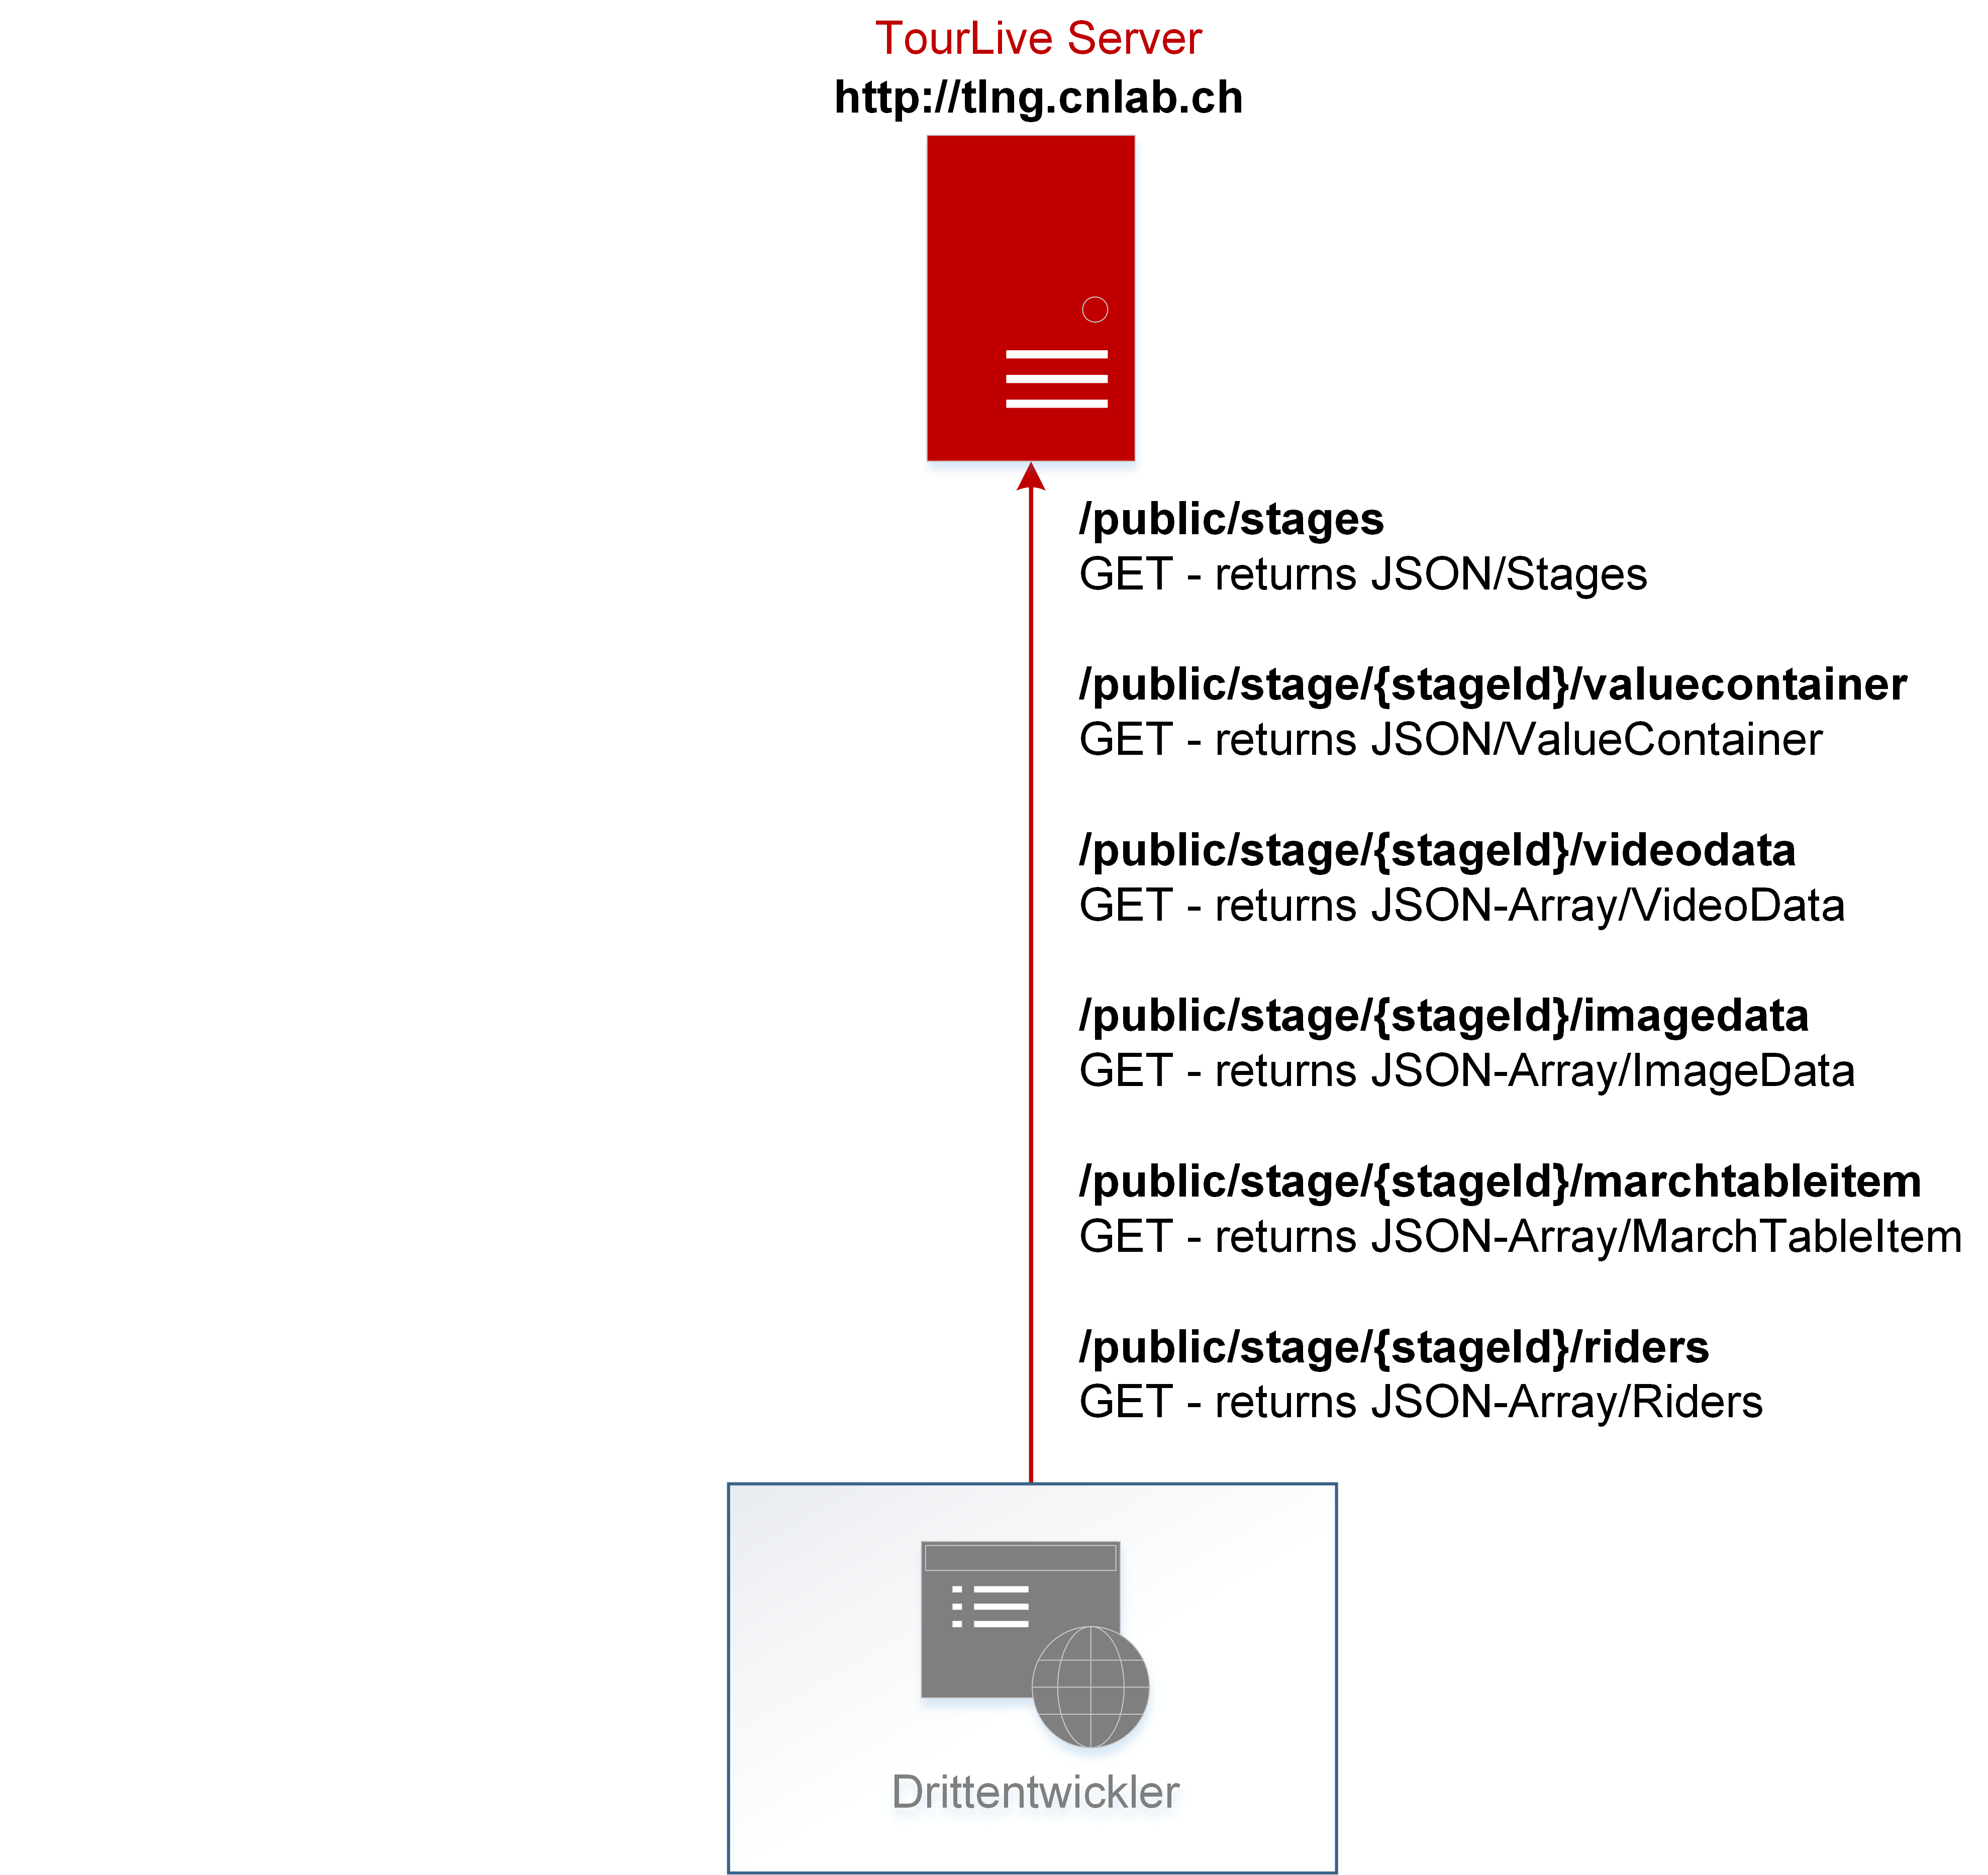
\includegraphics[width=130mm]{images/uebersicht_public_schnittstelle.png}
	\caption{Übersicht öffentliche Schnittstellen}
\end{figure}


\subsubsection{Etappen beim TourLive Server abfragen}
\begin{longtable}{ p{2.5cm} p{3.5cm} p{6cm}}
	\textbf{URL:} & \multicolumn{2}{l}{/public/stages} \\
	\textbf{Request:} & Method: & GET \\
		& Body: & <empty>\\
	\textbf{Response:} &  Header: & HTTP/1.1 200 OK \\
		& Content-Type: & application/json \\
		& Body: & JSON-Array 'Stages'\\
	\textbf{Bemerkung:} & \multicolumn{2}{p{10cm}}{Alle sichtbaren Etappen} 
\end{longtable}
\paragraph{Beispiel JSON - Array Stages}
\begin{figure}[H]
	\centering
	\lstinputlisting[language=json]{jsonfiles/stages.json}
	\caption{JSON-Struktur: Etappen}
\end{figure}

\subsubsection{ValueContainer beim TourLive Server abfragen}
\begin{longtable}{ p{2.5cm} p{3.5cm} p{6cm}}
	\textbf{URL:} & \multicolumn{2}{l}{/public/stage/\{stageId\}/valuecontainer} \\
	\textbf{Request:} & Method: & GET \\
		& Body: & <empty>\\
	\textbf{Response:} &  Header: & HTTP/1.1 200 OK \\
		& Content-Type: & application/json \\
		& Body: & JSON-Array 'ValueContainers'\\
	\textbf{Bemerkung:} & \multicolumn{2}{p{10cm}}{Alle ValueContainers einer Etappe}
\end{longtable}

\subsubsection{Bilderdaten beim TourLive Server abfragen}
\begin{longtable}{ p{2.5cm} p{3.5cm} p{6cm}}
	\textbf{URL:} & \multicolumn{2}{l}{/public/stage/\{stageId\}/imagedata} \\
	\textbf{Request:} & Method: & GET \\
		& Body: & <empty>\\
	\textbf{Response:} &  Header: & HTTP/1.1 200 OK \\
		& Content-Type: & application/json \\
		& Body: & JSON-Array 'ImageData'\\
	\textbf{Bemerkung:} & \multicolumn{2}{p{10cm}}{Alle ImageData Objekte zu dieser Etappe, nicht aber die eigentlichen Bilder. Die Bilder können aber mit dem Feld \textit{imageLocation} entweder direkt verlinkt oder heruntergeladen werden}
\end{longtable}

\paragraph{Beispiel JSON - ImageData}
\begin{figure}[H]
	\centering
	\lstinputlisting[language=json]{jsonfiles/imageData.json}
	\caption{JSON-Struktur: ImageData}
\end{figure}

\subsubsection{Videodaten beim TourLive Server abfragen}	
\begin{longtable}{ p{2.5cm} p{3.5cm} p{6cm}}
	\textbf{URL:} & \multicolumn{2}{l}{/public/stage/\{stageId\}/videodata} \\
	\textbf{Request:} & Method: & GET \\
		& Body: & <empty>\\
	\textbf{Response:} &  Header: & HTTP/1.1 200 OK \\
		& Content-Type: & application/json \\
		& Body: & JSON-Array 'VideoData'\\
	\textbf{Bemerkung:} & \multicolumn{2}{p{10cm}}{Alle VideoData Objekte zu dieser Etappe, nicht aber die eigentlichen Videosequenzen. Die Videos können aber mit dem Feld \textit{videoLocation} entweder direkt verlinkt oder heruntergeladen werden}
\end{longtable}

\paragraph{Beispiel JSON - VideoData}
\begin{figure}[H]
	\centering
	\lstinputlisting[language=json]{jsonfiles/videoData.json}
	\caption{JSON-Struktur: VideoData}
\end{figure}

\subsubsection{Marschtablle beim TourLive Server abfragen}
\begin{longtable}{ p{2.5cm} p{3.5cm} p{6cm}}
	\textbf{URL:} & \multicolumn{2}{l}{/public/stage/\{stageId\}/marchtableitem} \\
	\textbf{Request:} & Method: & GET \\
		& Body: & <empty>\\
	\textbf{Response:} &  Header: & HTTP/1.1 200 OK \\
		& Content-Type: & application/json \\
		& Body: & JSON-Array 'MarchTableItem'\\
	\textbf{Bemerkung:} & \multicolumn{2}{p{10cm}}{Die Marschtabelle ist aufgeteilt in Einheiten. Jede Reihe bedeutet eine Einheit. Pro Etappe können alle Marschtabelleneinheiten abgerufen werden.}
\end{longtable}

\paragraph{JSON Beispiel - Array MarchTableItem}
\begin{figure}[H]
	\centering
	\lstinputlisting[language=json]{jsonfiles/marchTableItems.json}
	\caption{JSON-Struktur: MarchTableItem}
\end{figure}

\subsection{Rennfahrer beim TourLive Server abfragen}
\begin{longtable}{ p{2.5cm} p{3.5cm} p{6cm}}	
	\textbf{URL:} & \multicolumn{2}{l}{/public/stage/\{stageId\}/riders} \\
	\textbf{Request:} & Method: & GET \\
		& Body: & <empty>\\
	\textbf{Response:} &  Header: & HTTP/1.1 200 OK \\
		& Content-Type: & application/json \\
		& Body: & JSON-Array 'Riders'\\
	\textbf{Bemerkung:} & \multicolumn{2}{p{10cm}}{Sämtliche Fahrer, welche dieser Etappe zugeordnet sind} \\ [1ex] 
\caption{TourLive Public API}
\end{longtable}

\paragraph{JSON Beispiel - Array Riders}
\begin{figure}[H]
	\centering
	\lstinputlisting[language=json]{jsonfiles/riders.json}
	\caption{JSON-Struktur: Riders}
\end{figure}



